\section{Système proie-prédateur de Lokta-Volterra}
Dans cette partie nous résolvons tous les systèmes par la méthode de Runge-Kutta exposée auparavant.

La capacité à prévoir les évolutions d'une population donnée grâce à des données environnementale a encouragé les travaux de scientifiques afin de proposer des modèles régissant ces évolutions. Les équations différentielles se revèlent être des outils fiables et pertinents pour modéliser ces variations de populations.

\subsection{Modèle de Malthus}
Malthus a proposé un modèle sur l'évolution des populations qui consiste à mesurer le taux de natalité $a$ et le taux de mortalité $b$ d'un population.

Il a établi l'équation différentielle suivante: 
\begin{equation}
\frac{\partial N(t)}{\partial t} = (a-b)N(t)
\end{equation}

On peut poser $\gamma = a-b$ qui est le taux intrinsèque d'accroissement naturel.

Les 3 types d'évolutions que l'on peut trouver dépendent du signe de $\gamma$, comme montré à la figure~\vref{fig:malthus}.

\begin{figure}
\centering
\begin{subfigure}[b]{.3\textwidth}
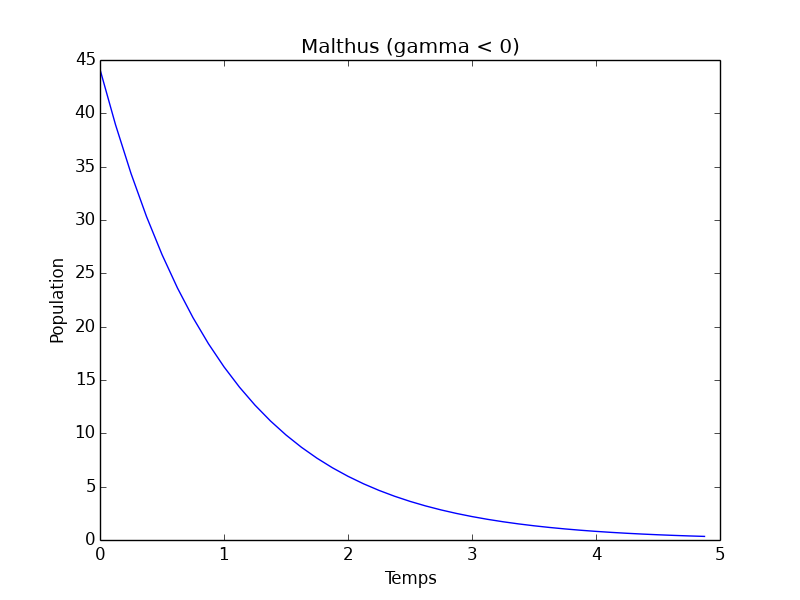
\includegraphics[width=\textwidth]{mathusinf0}
\end{subfigure}
\begin{subfigure}[b]{.3\textwidth}
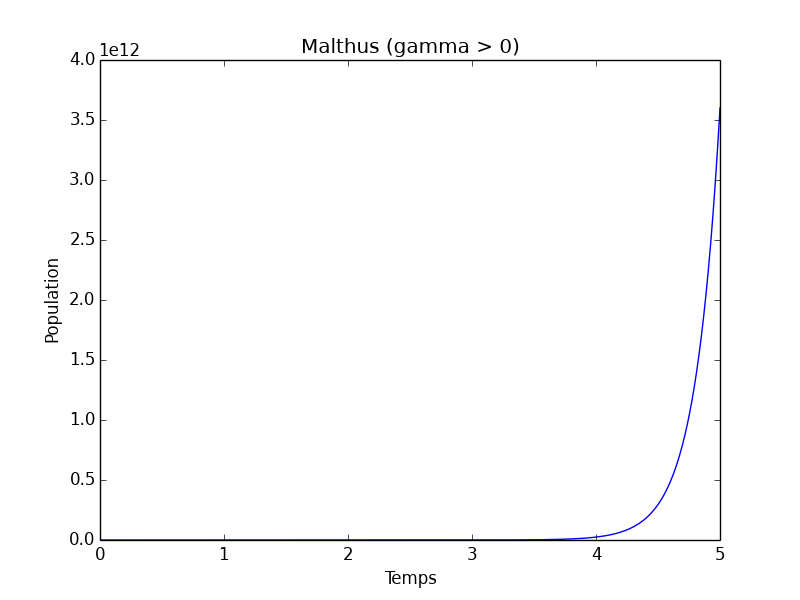
\includegraphics[width=\textwidth]{mathussup0}
\end{subfigure}

\caption{Malthus}
\label{fig:malthus}
\end{figure}

\subsection{Modèle de Verhulst}
Verhulst a proposé un modèle plus complexe pour modéliser l'évolution des populations. Dans ce modèle, il prend en compte le taux de croissance $\gamma$ et la capacité d'acceuil $\kappa$ de l'environnement.

Nous avons l'équation suivante:
\begin{equation}
\frac{\partial N(t)}{\partial t} = \gamma N(t)(1 - \frac{N(t)}{\kappa})
\end{equation}
 Ce problème peut être modélisé comme un problème de Cauchy moyennant l'ajout d'une condition initiale telle que le nombre d'invidu à t = 0.
 Cependant cette modélisation demeure simpliste de part le fait que seule la capacité d'acceuil de l'environnement soit un facteur limitant, ne tenant pas en compte l'intervention d'autres espèces. C'est pour cela que nous allons nous intéresser maintenant au système proie prédateur de Lokta-Volterra.
 
\begin{figure}
\centering
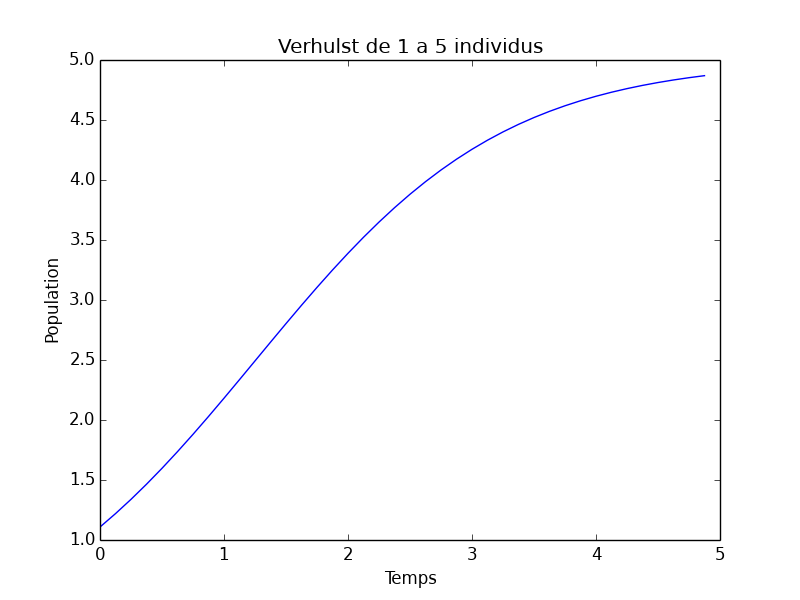
\includegraphics[width=.3\textwidth]{verhulst}

\caption{Verhulst}
\label{fig:verhulst}
\end{figure}
 
\subsection{Modèle de Lotka-Volterra}


Le modèle de population Lotka-Volterra considère l'interaction entre deux populations et nécessite deux constantes pour chaque espèce. Nous faisons l'hypothèse que les proies ne peuvent pas mourir de faim. Leur taux de mortalité est alors uniquement relié par la constante $\beta$ à la probabilité d'être mangé par un predateur, et donc au nombre de predateurs.
Une seconde constante  $\alpha$ va permettre de quantifier la rapidité de reproduction de l'espece proie, ce qui nous donne une premiere équation (3). Pour les predateurs , nous supposons que leur durée de vie est proportionnelle au nombre de leurs proies selon un coefficient  $\delta$ et nous caracterisons leur taux de mortalite par une constante $\gamma$
ce qui nous donne l'équation (4).

Nous obtenons ainsi le systeme différentiel :
\begin{equation}
\frac{\partial x(t)}{\partial t} = x(\alpha - \beta y)
\end{equation}
\begin{equation}
\frac{\partial y(t)}{\partial t} = y(\delta x - \gamma)
\end{equation}

Ce système admet une solution analytique, nous allons donc fixer des constantes pour la résoudre de manière approchée et comparer avec la solution analytique.

On peut obtenir la solution figure~\vref{fig:lv}
, avec les paramètres (1, 1, 1, 1) et la condition initiale (1.5, 1.5).

\begin{figure}
\centering
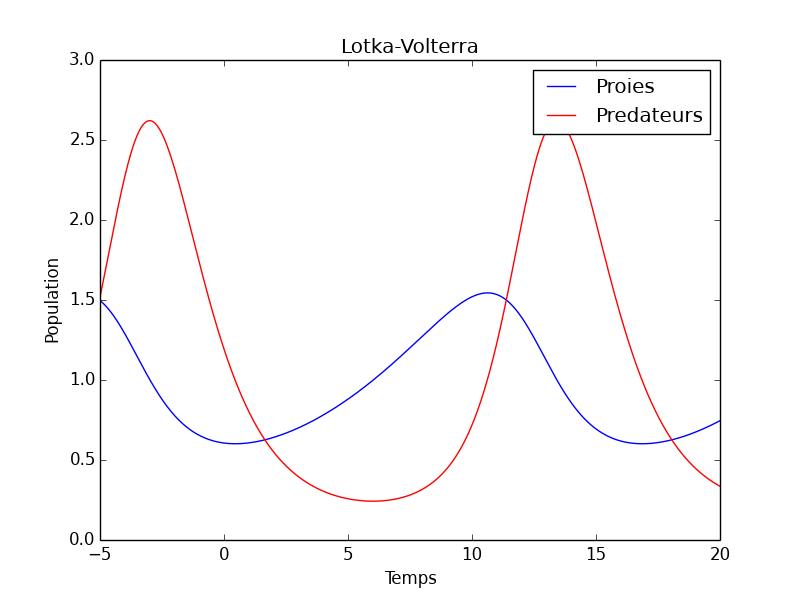
\includegraphics[width=.3\textwidth]{lotkavolterra}

\caption{Lotka-Volterra}
\label{fig:lv}
\end{figure}

La trajectoire correspondante (équation paramétrique) est tracée à la figure~\vref{fig:trajectoire}.

\begin{figure}
\centering
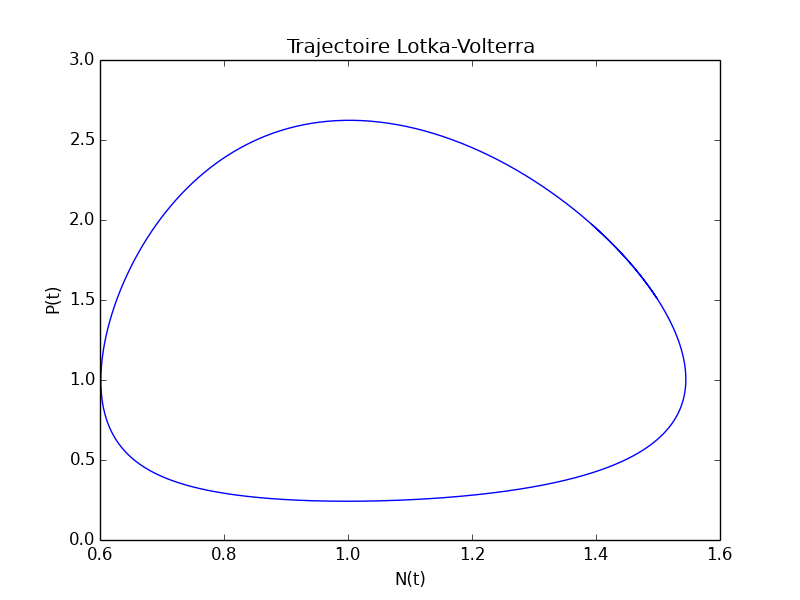
\includegraphics[width=.3\textwidth]{trajectoire}

\caption{Trajectoire}
\label{fig:trajectoire}
\end{figure}

On fait alors apparaitre des solutions périodiques, sauf dans le cas ou les deux populations sont constantes. Ces solutions correspondent aux points singuliers du systèmes : $N(t) = P(t) = 0$ ou $N(t) = \frac{d}{c}, P(t) = \frac{a}{b}$.

\begin{figure}
\centering
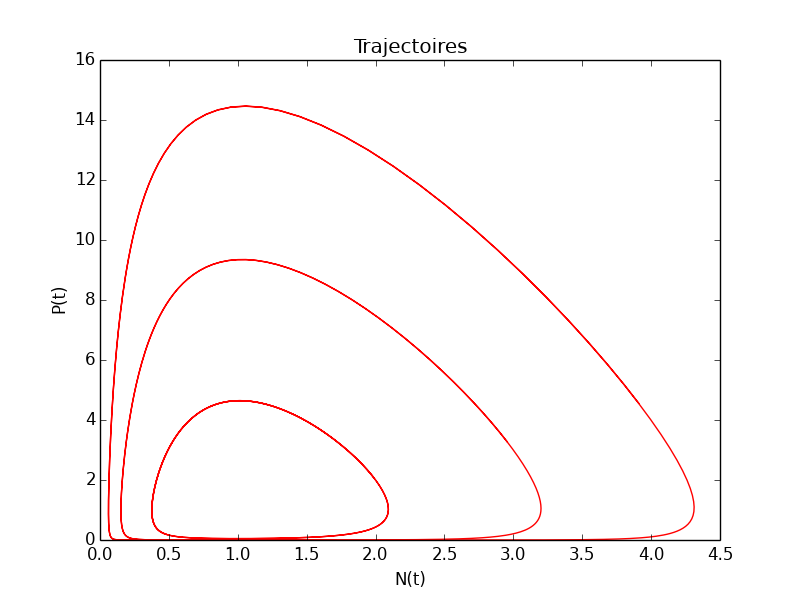
\includegraphics[width=.3\textwidth]{trajectoires}

\caption{Trajectoires}
\label{fig:trajectoires}
\end{figure}
